\documentclass[notes=show]{beamer}

\usepackage{comment}
\usepackage{default}
\usepackage[utf8]{inputenc}
\usepackage{listings}
\usepackage{graphicx}

\graphicspath{{./images/}}

\definecolor{OliveGreen}{cmyk}{0.64,0,0.95,0.40}
\definecolor{Gray}{gray}{0.5}

\lstset{
    language=C,
    basicstyle=\ttfamily\scriptsize,
    keywordstyle=\color{OliveGreen},
    commentstyle=\color{Gray},
    captionpos=b,
    breaklines=true,
    breakatwhitespace=false,
    showspaces=false,
    showtabs=false,
    numbers=left,
}

\title{An Efficient Parallel Signal Temporal Logic Implementation}
\author{
	Bernhard Denner,
	Jakob Gruber,
	Mino Sharkhawy
}

\begin{document}

\maketitle

\begin{frame}
\frametitle{Signal Temporal Logic}
% Very brief recap
\end{frame}

\begin{frame}
\frametitle{Objectives}
Parallelize all STL operators!
\end{frame}

\begin{frame}
\frametitle{Work Division}
\begin{itemize}
\item A lightweight on-the-fly plan
\item Organized through the bitbucket issue tracker
\item Jakob: Test suite, AND, UNTIL
\item Mino: EVTL, BEVTL
\item Bernhard: Benchmark framework, Matlab integration
\end{itemize}
\end{frame}

\begin{frame}
\frametitle{Testing and Benchmarks}
\begin{itemize}
\item CTest: Integration into build system
\item Check: Test framework
\item One test suite per operator
\item Comparison against Breach results
\end{itemize}
\end{frame}

\begin{frame}
\frametitle{Initial Plan}
% What did we initially want to do?
\begin{itemize}
\item Primitive operators
\begin{itemize}
\item NOT - done
\item AND - done
\item unbounded EVTL - done
\item unbounded UNTIL - partially done
\item bounded EVTL - done
\end{itemize}
\item Test suite - done
\item Benchmarking - done
\item Parser integration - not done
\item Optimization - not done
\end{itemize}
\end{frame}

\begin{frame}
\frametitle{Problems}
\begin{itemize}
\item Getting the breach reference implementation to work and to produce results for
        comparison was difficult.
\item Some operators very hard to parallelize
\begin{itemize}
\item Fully parallelize UNTIL needs infinite amount of memory
\item Even partial parallelization of UNTIL very difficult
\item Running time of parallel BEVTL depends on the window size
\end{itemize}
\item Floating point calculations very inaccurate, best accuracy: $5*10^{-5}$.
\end{itemize}
\end{frame}

\begin{frame}
\frametitle{Results}
\begin{itemize}
\item NOT trivially parallelizable
\item AND, EVTL involved, but possible in $O(f(n,p))$
\item UNTIL mostly possible, but one sequential part remains
\item BEVTL parallelizable, but dependent on window size $O(f(n,p,w))$
\end{itemize}
% Also, why we ended up with less than planned, what were the difficulties?
\end{frame}

\begin{frame}
\frametitle{Benchmarks - AND}
\begin{figure}[H]
    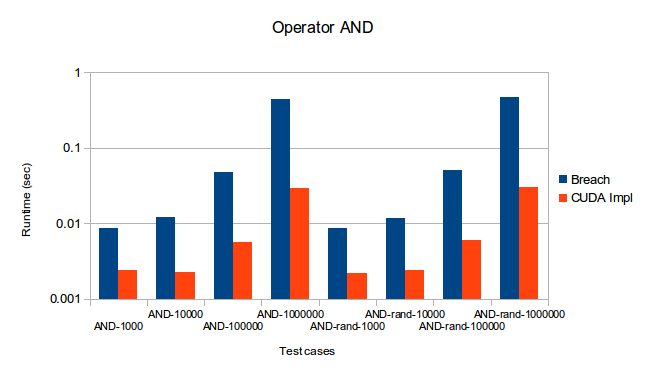
\includegraphics[scale=0.5]{bm_and.png}
    \caption{
        \label{fig:bm_and}
        Benchmark result: AND Operator}
\end{figure}
\end{frame}

\begin{frame}
\frametitle{Benchmarks - EVTL}
\begin{figure}[H]
    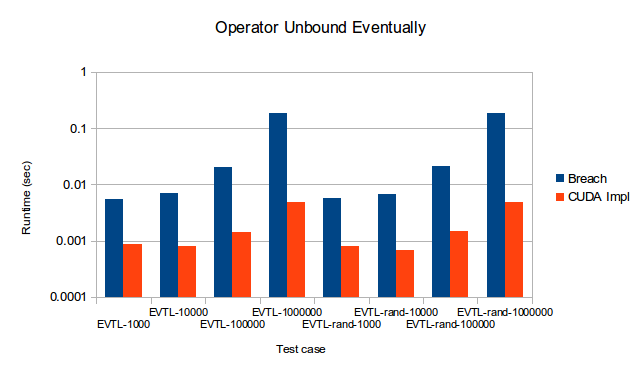
\includegraphics[scale=0.5]{bm_evtl.png}
    \caption{
        \label{fig:bm_evtl}
        Benchmark result: EVTL Operator}
\end{figure}
\end{frame}

\begin{frame}
\frametitle{Benchmarks - UNTIL}
\begin{figure}[H]
    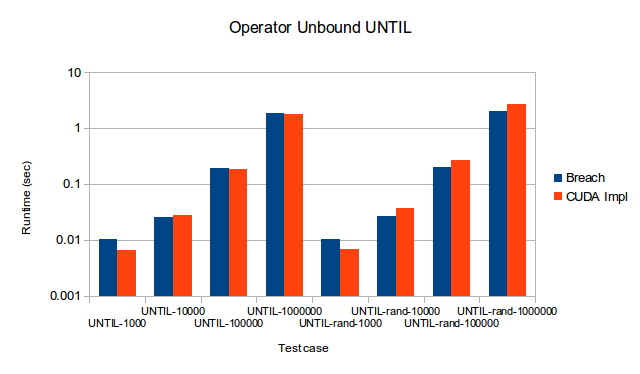
\includegraphics[scale=0.5]{bm_until.png}
    \caption{
        \label{fig:bm_until}
        Benchmark result: UNTIL Operator}
\end{figure}
\end{frame}

\begin{frame}
\frametitle{Benchmarks - BEVTL}
\begin{figure}[H]
    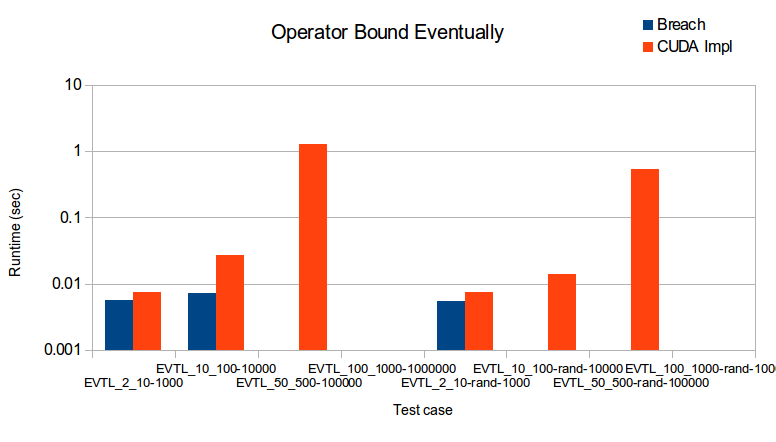
\includegraphics[scale=0.5]{bm_bevtl.png}
    \caption{
        \label{fig:bm_bevtl}
        Benchmark result: BEVTL Operator}
\end{figure}
\end{frame}

\begin{frame}
\frametitle{Lessons Learned}
\begin{itemize}
\item Create benchmarks at the beginning
\item Floating point arithmetic
\item Simple POC before implementation
\item Ensure task is possible before barging in
\end{itemize}
\end{frame}

\begin{frame}
\frametitle{Future Tasks}
\begin{itemize}
\item Completely parallel UNTIL, EVTL not dependent on window size
\item Multi-GPU
\item Optimizations
\item Processing entire formulas
\item Arbitrary expressions in input formulas
\end{itemize}
\end{frame}

\end{document}
